\chapter{弦、引力、緊緻化與 T 對偶}

\lectureoverview{點粒子幾乎可以在任何光滑幾何上自洽地運動，量子弦卻不行。弦有無窮多個零點振盪，會逐步探測靶空間中愈來愈短的尺度；隨著這些振盪逐一納入，有效幾何也會改變。要求這個過程達到不動點，便得到\(R_{\mu\nu}=0\)，也就是真空愛因斯坦方程。接著，我們從這項一致性條件轉向緊緻化。一個圓同時具有 Kaluza--Klein 動量態與弦的纏繞態；將兩者互換，半徑為\(R\)的圓便與半徑為\(\alpha'/R\)的圓等價。}

\section{作為選擇原理的一致性}

有兩個問題需要回答：為什麼弦理論中會有引力？為什麼弦理論比點粒子力學嚴格得多？這其實是同一個問題。背景幾何只有在弦能於其中傳播，且結果不會任意依賴我們對弦分辨得多精細時，才是可接受的。

先看一個對照問題：受限於光滑彎曲曲面上的點粒子。經典情況下，它沿著測地線運動；測地線是直線在曲面內部的對應概念。我們可以用許多短線段近似其運動，寫出差分方程，再令線段長度趨近於零。所得常微分方程具有明確的連續極限。

量子力學改變的是對歷史的求和方式，結論卻不變。我們不再選定一條經典路徑，而是對曲面上的路徑求振幅總和。時間同樣可以切分成許多小步；取極限後，也可以用彎曲位形空間上的Schr\"odinger方程來描述。對光滑曲面而言，這個極限會收斂到確定的傳播子與能譜。

\begin{figure}[H]
  \centering
  \includegraphics[width=0.72\textwidth]{lecture_09_figure_01.png}
  \caption{曲面上的光滑路徑，以及時間切片量子求和所涵蓋的鋸齒狀路徑。兩者都位於靶曲面上，並由其內在幾何描述。}
  \lectureframe{00:05:10}
  \label{fig:l09-particle-paths}
\end{figure}

\begin{classroomqa}
\audiencequestion{在路徑積分中，是否所有路徑都必須留在曲面上？\lecturetimestamp{00:05:39}}
\lecturerresponse{是。曲面就是粒子的位形空間，不是嵌在更大空間中的薄片，讓粒子可以穿過外部空間抄近路。每個中間點都必須位於曲面上，所有長度與作用量都以曲面的內在度規計算。}
\end{classroomqa}

對弦而言，相應的問題更難。弦不能只用質心位置來描述；它還有無窮多個振子模。因此，提高解析度也就意味著納入更多動力學自由度。只有在逐步納入這些振子模時，觀測量仍趨近某個極限，理論才是一致的。

\section{球面上的點粒子}

球面是最簡單的彎曲測試幾何。設球面半徑為\(R\)，先將質量為\(m\)的粒子放在球面上。若粒子沿大圓運動，
\begin{equation}
  E=\frac{1}{2}mv^2=\frac{p^2}{2m},
  \qquad
  L=pR.
  \label{eq:l09-particle-energy}
\end{equation}
因此，
\begin{equation}
  E=\frac{L^2}{2mR^2}
   =\frac{L^2}{2I},
  \qquad
  I=mR^2.
  \label{eq:l09-rotor-energy}
\end{equation}
半徑透過轉動慣量進入計算。將角動量量子化後，便得到熟悉的剛性轉子能譜，而且完全不需要紫外截斷。

\begin{figure}[H]
  \centering
  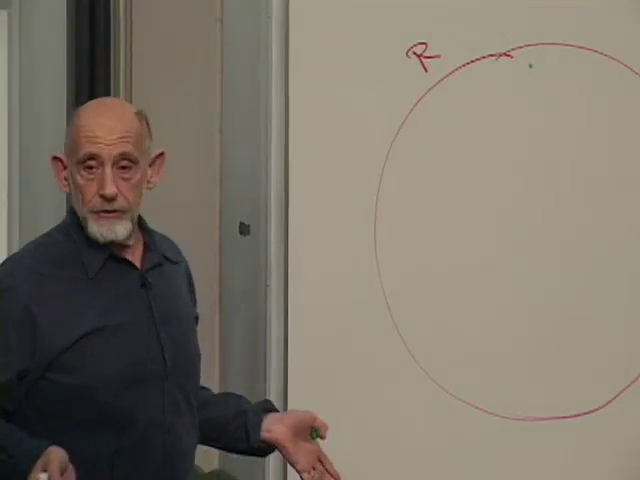
\includegraphics[width=0.74\textwidth]{lecture_09_figure_02.png}
  \caption{點粒子的對照計算：\(p^2/(2m)=L^2/(2mR^2)=L^2/(2I)\)。}
  \lectureframe{00:11:25}
  \label{fig:l09-sphere-rotor}
\end{figure}

這個毫無困難的例子很重要。問題不在曲率本身，而是在曲率與弦的量子內部延展性耦合時才會出現。

\section{真空中的弦並非點狀}

考慮開弦的一個橫向座標，並扣除質心位置。這裡採用的振子展開式僅為示意：
\begin{equation}
  X(\sigma)-X_{\mathrm{cm}}
  \sim
  \sum_{n=1}^{\infty}
  \frac{a_n+a_n^\dagger}{\sqrt n}\cos(n\sigma).
  \label{eq:l09-mode-expansion}
\end{equation}
關鍵成分是餘弦模、振子算符，以及因子\(1/\sqrt n\)。在討論尺寸時，精確的歸一化並不重要。
\editorialnote{精確展開式還包含依約定而定的\(\alpha'\)因子、數值常數，以及不同的振子記號。方程\eqref{eq:l09-mode-expansion}只保留紫外估算所需的依賴關係，與黑板上的推導相同。}

\begin{figure}[H]
  \centering
  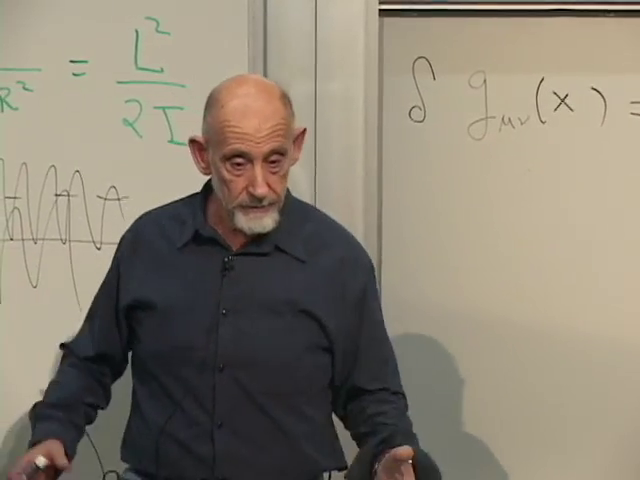
\includegraphics[width=0.78\textwidth]{lecture_09_figure_03.png}
  \caption{振子展開的結構，以及將其平方後得到的雙重求和。}
  \lectureframe{00:15:20}
  \label{fig:l09-string-modes}
\end{figure}

在振子真空態中，相對於質心的距離平方為
\begin{align}
  \expect{\bigl(X(\sigma)-X_{\mathrm{cm}}\bigr)^2}_0
  &\sim
  \sum_{n,m\geq1}
  \frac{\cos(n\sigma)\cos(m\sigma)}{\sqrt{nm}}\notag\\
  &\qquad\times
  \bra{0}(a_n+a_n^\dagger)\notag\\
  &\hspace{6em}\times(a_m+a_m^\dagger)\ket{0}.
  \label{eq:l09-size-double-sum}
\end{align}
大多數項都會消失：兩個湮滅算符作用於右矢後為零；兩個產生算符作用後所得的態與左矢正交；依此排序，先產生再湮滅的算符組合，其真空期望值也為零。剩下的收縮項為
\begin{equation}
  \bra{0}a_n a_m^\dagger\ket{0}=\delta_{nm}.
  \label{eq:l09-vacuum-contraction}
\end{equation}

\begin{figure}[H]
  \centering
  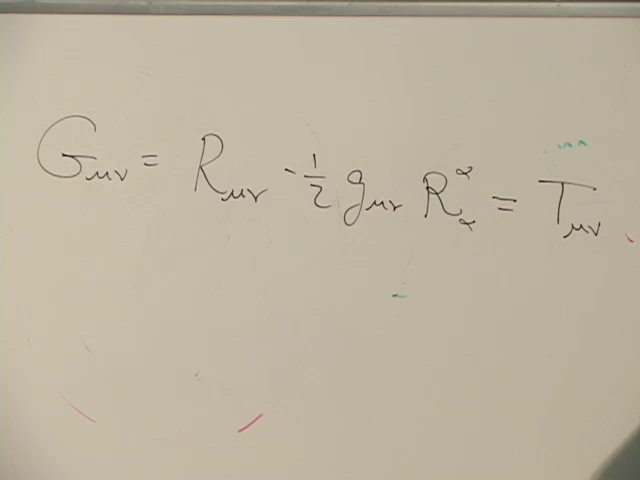
\includegraphics[width=0.74\textwidth]{lecture_09_figure_04.png}
  \caption{剩下的真空收縮使雙重振子求和化為單一求和。}
  \lectureframe{00:20:10}
  \label{fig:l09-vacuum-contraction}
\end{figure}

因此
\begin{equation}
  \expect{\bigl(X(\sigma)-X_{\mathrm{cm}}\bigr)^2}_0
  \sim
  \sum_{n=1}^{\infty}\frac{\cos^2(n\sigma)}{n}.
  \label{eq:l09-size-single-sum}
\end{equation}
在弦上的一般位置，或對\(\sigma\)取平均後，\(\cos^2(n\sigma)\)的貢獻約為\(1/2\)。若模式截斷為\(N\)，則
\begin{equation}
  \expect{\bigl(X-X_{\mathrm{cm}}\bigr)^2}_{0,N}
  \sim
  \frac{1}{2}\sum_{n=1}^{N}\frac{1}{n}
  =\frac{1}{2}\log N+O(1).
  \label{eq:l09-logarithmic-size}
\end{equation}

\begin{figure}[H]
  \centering
  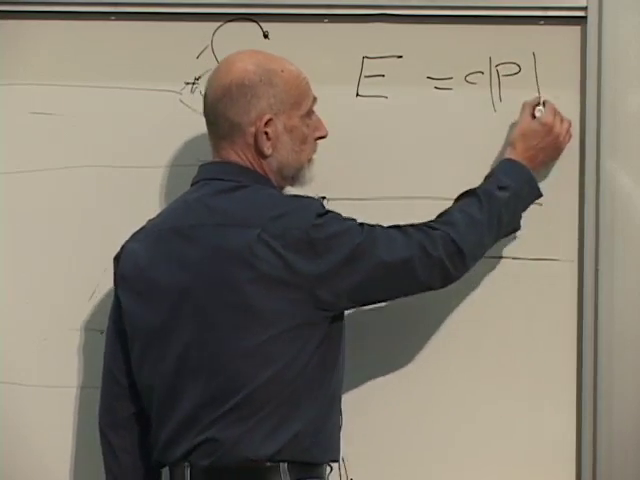
\includegraphics[width=0.72\textwidth]{lecture_09_figure_05.png}
  \caption{黑板上的推導得到控制基態展寬的調和級數。}
  \lectureframe{00:22:05}
  \label{fig:l09-harmonic-size}
\end{figure}

例如只保留前二十五個模式，會得到一個有限但模糊的物體；然而它還不是連續弦。移除截斷後，均方展寬會按對數增長。這不代表平直空間中的弦理論不一致。在平直空間中，質心運動與振子運動彼此分離，而物理振幅中的精細抵消會維持預期的局域性。尺寸增長是一項警訊；曲率則告訴我們這項警訊是否會演變成問題。

\section{內部展寬如何改變幾何}

把弦放在球面的北極附近。關閉所有振子時，它的行為就像剛才討論的點粒子。逐步納入較高模式後，弦會形成在球冠上散開的漲落結構。它的中心仍可繞著球面運動，但現在參與決定轉動慣量的，是一個延展物體。

若轉軸通過球心與兩極，
\begin{equation}
  I=\int r_\perp^2\,dm,
  \label{eq:l09-extended-inertia}
\end{equation}
其中\(r_\perp\)是弦上一小段到該軸的垂直距離。軌道赤道上的點具有最大的相關力臂；弦上向轉軸垂下的部分，貢獻則較小。在總質量固定時，有效轉動慣量因此降低：
\begin{equation}
  I_{\mathrm{eff}}<mR^2.
  \label{eq:l09-inertia-reduction}
\end{equation}
所以轉動能量看起來就像是位於較小球面上的點狀物體所具有的轉動能量：
\begin{equation}
  E_{\mathrm{rot}}
  =\frac{L^2}{2I_{\mathrm{eff}}}
  \equiv \frac{L^2}{2mR_{\mathrm{eff}}^2},
  \qquad R_{\mathrm{eff}}<R.
  \label{eq:l09-effective-radius}
\end{equation}

\begin{classroomqa}
\audiencequestion{如果弦散布到更大的區域，為什麼轉動慣量會趨近於零？\lecturetimestamp{00:33:23}}
\lecturerresponse{這裡說的是逐步粗粒化後的有效描述，並不是說原本的延展分布會立刻變成零慣量。第一層模式使點粒子成為一團模糊的物體，其運動彷彿發生在較小的球面上。下一層模式解析這團物體內部的結構，並再次進行相同的重整化。反覆比較下去，有效半徑便會逐步縮小。}
\end{classroomqa}

\begin{figure}[H]
  \centering
  \includegraphics[width=0.72\textwidth]{lecture_09_figure_06.png}
  \medskip

  \begin{adjustbox}{max width=\linewidth}
  \begin{tikzpicture}[x=1cm,y=1cm,>=Latex]
    \draw[thick] (0,0) circle (2.15);
    \draw[dashed] (0,-2.55) -- (0,2.55);
    \draw[blue!65!black,thick]
      (-0.22,2.05)
      .. controls (-1.22,1.75) and (-1.52,1.08) .. (-1.06,0.44)
      .. controls (-0.55,-0.10) and (0.35,0.02) .. (1.10,0.68)
      .. controls (1.48,1.12) and (1.16,1.80) .. (0.20,2.05);
    \draw[red!70!black,dashed] (0,0) circle (1.25);
    \draw[->] (2.70,1.55) -- (4.05,1.55);
    \node[align=center] at (3.37,1.98) {add shorter\\modes};
    \draw[thick] (6.15,0) circle (1.25);
    \draw[dashed] (6.15,-1.65) -- (6.15,1.65);
    \draw[blue!65!black,thick]
      (6.00,1.18)
      .. controls (5.42,0.88) and (5.46,0.25) .. (6.02,-0.06)
      .. controls (6.46,-0.28) and (6.90,0.45) .. (6.28,1.18);
    \node at (0,-3.00) {sphere of radius \(R\)};
    \node at (6.15,-2.05) {effective radius \(R_{\mathrm{eff}}\)};
  \end{tikzpicture}
  \end{adjustbox}
  \caption{黑板上的北極弦，以及有效半徑論證的清晰重建。虛線內圓表示有效幾何，不是球面內部的另一個實體殼層。}
  \lectureframe{00:35:15}
  \label{fig:l09-shrinking-sphere}
\end{figure}

這是重整化群的敘述。有限截斷下，弦是一團具有有限內部解析度的物體；提高截斷會改變這團物體的力學。在正曲率球面上，每增加一層模式，從長距離運動推得的背景就會縮小。如果這個結果始終無法穩定下來，該背景上便不存在與截斷無關的弦理論。

\section{度規必須達到不動點}

現在將球面換成一般的靶空間度規\(g_{\mu\nu}(x)\)。將一薄層振子模式積分掉，會使度規改變；這項改變是局域的對稱二階張量。它在平直空間中必須消失，而且須從度規的二階導數開始。在最低階，協變性留下裡奇張量作為相關候選：
\begin{equation}
  \frac{\partial g_{\mu\nu}}{\partial\log\Lambda}
  =-C\,R_{\mu\nu}+\cdots ,
  \qquad C>0
  \label{eq:l09-ricci-flow}
\end{equation}
其流動方向與幾何論證所採用的粗粒化方向一致。因此，正曲率會使球面向內縮，正如預期。
\editorialnote{歸一化與符號取決於重整化參數是朝紫外端還是紅外端增加。在慣用的世界面記號中，最低階的度規貝塔函數為\(\beta^g_{\mu\nu}=\alpha'R_{\mu\nu}+\cdots\)。此處採用的不變敘述是：截斷獨立性要求貝塔函數為零，因此在這個階數也要求\(R_{\mu\nu}\)為零。}

\begin{figure}[H]
  \centering
  \includegraphics[width=0.76\textwidth]{lecture_09_figure_07.png}
  \caption{度規的變化以負的裡奇張量示意表示，旁邊畫著一條平滑曲線。}
  \lectureframe{00:43:00}
  \label{fig:l09-ricci-flow-board}
\end{figure}

\begin{classroomqa}
\audiencequestion{振子截斷\(N\)在這個流方程中出現在哪裡？\lecturetimestamp{00:43:38}}
\lecturerresponse{它就是尺度變數。最高納入模式的變化會使弦尺寸的總和呈對數變化，因此自然的演化參數是\(\log N\)，也就是等價的\(\log\Lambda\)。方程\eqref{eq:l09-ricci-flow}描述由一層對數模式殼層造成的無窮小變化。}
\end{classroomqa}

可接受的背景是這個流的固定點。在最低階，
\begin{equation}
  \boxed{R_{\mu\nu}=0.}
  \label{eq:l09-ricci-flat}
\end{equation}
裡奇平坦並不表示黎曼張量的每個分量都為零。例如，真空中的引力波可以具有非零曲率，同時滿足\(R_{\mu\nu}=0\)。

\subsection{同一條件也是真空愛因斯坦方程}

略去慣用常數後，愛因斯坦方程為
\begin{equation}
  G_{\mu\nu}
  \equiv
  R_{\mu\nu}-\frac12 g_{\mu\nu}R
  =T_{\mu\nu}.
  \label{eq:l09-einstein}
\end{equation}

\begin{figure}[H]
  \centering
  \includegraphics[width=0.78\textwidth]{lecture_09_figure_08.png}
  \caption{黑板上的愛因斯坦張量與應力張量。}
  \lectureframe{00:47:15}
  \label{fig:l09-einstein-board}
\end{figure}

真空中\(T_{\mu\nu}=0\)。在\(D\)維時空中取跡，可得
\begin{equation}
  0=g^{\mu\nu}G_{\mu\nu}
   =\left(1-\frac{D}{2}\right)R.
  \label{eq:l09-einstein-trace}
\end{equation}
當\(D\neq2\)時，\(R=0\)；再代回\eqref{eq:l09-einstein}，便得到\(R_{\mu\nu}=0\)。因此，弦不再依賴截斷的條件，就是真空引力場方程。引力並非額外附加到理論中的，而是維持一致性所必須付出的代價。

\emph{真空}一詞不代表什麼都沒有發生，而是指該區域沒有應力能量源。無源的馬克士威方程允許電磁波，無源的愛因斯坦方程也允許引力波。即使裡奇張量為零，幾何仍然可以隨時間演化。

\begin{classroomqa}
\audiencequestion{這個條件和共形不變性有關嗎？\lecturetimestamp{00:52:20}}
\lecturerresponse{有關，儘管錄音中有一部分問題沒有記錄下來。相關的對稱性是量子\emph{世界面}理論的共形不變性。要求世界面尺度反常消失，便會使度規貝塔函數為零。這不能與要求時空本身具有共形不變性混為一談。}
\end{classroomqa}

還有第二項一致性條件：世界面共形不變性也會決定臨界時空維度，超弦為十維，玻色弦為二十六維。因此，裡奇平坦並非全部要求，但它是最直接呈現愛因斯坦方程的部分。

\section{緊緻維度，而非消失的維度}

超弦背景有九個空間維度和一個時間維度。我們的宏觀世界只呈現三個大型空間方向，因此另外六個空間維度必須隱藏起來，或以其他方式使我們在一般尺度下無法接觸。緊緻化讓它們仍是真實的維度，只是範圍有限且很小。

\begin{classroomqa}
\audiencequestion{如果不同觀測者各自帶著不同的時鐘，這是否就代表有不只一個時間維度？\lecturetimestamp{00:56:59}}
\lecturerresponse{不是。多個時鐘只是多種測量單一時空座標的儀器，並不會創造出彼此獨立的類時方向。此處討論的額外維度是空間維度。熟知的量子與因果架構並未提供一套可與之相當、且具有多個局域時間方向的一致理論，因此多個時間方向不在這個緊緻化模型的範圍內。}
\end{classroomqa}

想像一群生物相信自己的世界是一條線。在低解析度下，它們只能前後移動。但用足夠強的顯微鏡觀察，會發現這條線其實是非常細的圓柱。小生物除了可以沿著圓柱的長度移動，也能繞著圓柱的圓周移動。第二個方向一直都在，只是圓周太小，粗略的探測無法分辨。

\begin{figure}[H]
  \centering
  \includegraphics[width=0.78\textwidth]{lecture_09_figure_09.png}
  \caption{狹窄的圓柱，以及繞著其隱藏圓周方向前進的軌跡。}
  \lectureframe{01:01:00}
  \label{fig:l09-hidden-cylinder}
\end{figure}

圓柱可以表示成一條帶狀區域，並將上下兩邊識別為同一邊。穿過上邊後，會從下邊相同的縱向位置接續出現；兩邊都不是實際的邊界。同樣的操作也能在兩個方向上進行：將矩形的左右兩邊識別在一起，再將上下兩邊識別在一起，結果便是二維環面。

\begin{figure}[H]
  \centering
  \includegraphics[width=0.76\textwidth]{lecture_09_figure_10.png}
  \medskip

  \begin{tikzpicture}[x=0.82cm,y=0.82cm,>=Latex]
    \draw[thick] (0,0) rectangle (4,2.15);
    \draw[blue!65!black,->] (0,2.48) -- (4,2.48);
    \draw[blue!65!black,->] (4,-0.34) -- (0,-0.34);
    \node at (2,-0.82) {one periodic direction};
    \draw[thick] (6.1,0) rectangle (10.1,2.15);
    \draw[blue!65!black,->] (6.1,2.48) -- (10.1,2.48);
    \draw[blue!65!black,->] (10.1,-0.34) -- (6.1,-0.34);
    \draw[red!70!black,->] (5.76,0) -- (5.76,2.15);
    \draw[red!70!black,->] (10.44,2.15) -- (10.44,0);
    \node at (8.1,-0.82) {two periodic directions};
  \end{tikzpicture}
  \caption{黑板上的板狀區域，以及清楚的基本域描述。識別一對邊可得到圓柱；識別兩對邊則得到環面。}
  \lectureframe{01:04:40}
  \label{fig:l09-periodic-identification}
\end{figure}

環面首先是一種拓撲空間，其次才是三維空間中形似甜甜圈的曲面。將環面剪開一次會得到圓柱，再剪一次便成為矩形，但必須保留原先邊界的識別方式。在這個矩形上可以賦予平坦度規，因此形成的平坦環面在局部具有零黎曼曲率，當然也就是裡奇平坦。

矩形上的直線軌跡穿越已識別的邊界後，仍會沿直線延續。如果斜率是兩個週期長度的有理數比例，軌跡最終會閉合；若比例是無理數，軌跡便永不閉合，而會在環面上稠密分布。

\begin{figure}[H]
  \centering
  \includegraphics[width=0.76\textwidth]{lecture_09_figure_11.png}
  \caption{基本域中反覆出現的直線線段，代表環面上一條連續不斷的軌跡。}
  \lectureframe{01:11:00}
  \label{fig:l09-torus-trajectory}
\end{figure}

高維環面也以相同方式構成。將立方體的每一對相對面識別在一起，便得到三維環面；六個緊緻方向則可用六維環面建模。無須試圖把這些物體全都嵌入一般的三維空間；以面識別來描述，既是內在的，也已足夠完整。

\begin{classroomqa}
\audiencequestion{額外維度是否必然要捲曲成閉合的形狀？\lecturetimestamp{01:15:03}}
\lecturerresponse{這不是定理。額外維度也可以是非緊緻的，但如此一來，通常就會在我們觀測到的長距離世界中呈現為另一個大型方向。緊緻化是讓額外維度與它們表面上不存在的現象相容，最簡單的方法。自然界為何選擇某一種特定的緊緻化，則是另一個動力學問題。}
\end{classroomqa}

\begin{classroomqa}
\audiencequestion{為什麼要假設看不見的維度是以這種方式捲曲起來的一般空間方向，而不是完全不同的事物？\lecturetimestamp{01:15:51}}
\lecturerresponse{因為這是一個明確且可求解的假設，而不是因為它已被證明是描述自然界的唯一方式。緊緻空間流形讓我們能構造一致的例子，並計算它們的能譜。更奇特的可能性也必須做到同樣的事，才能成為值得考慮的選項。}
\end{classroomqa}

\begin{classroomqa}
\audiencequestion{熟悉的甜甜圈形環面上的距離，看起來不像矩形上的距離。這裡說的是哪一種幾何？
\lecturetimestamp{01:18:11}}
\lecturerresponse{\emph{環面}這個名稱決定的是邊界識別方式，而不是唯一的度規。嵌入三維空間的甜甜圈形曲面，承襲了三維空間所誘導的彎曲度規；週期性識別邊界的矩形則帶有平坦度規。兩者拓撲相同，幾何不同；此處討論的簡單緊緻化採用平坦度規。}
\end{classroomqa}

\section{平坦環面的形狀參數}

即使是平坦的二維環面，也不只有一種。它的基本平行四邊形有整體面積、長寬比與剪切量。改變這些參數會改變距離，進而改變能譜，但不會改變拓撲。

\begin{figure}[H]
  \centering
  \includegraphics[width=0.74\textwidth]{lecture_09_figure_12.png}
  \medskip

  \begin{tikzpicture}[x=0.9cm,y=0.9cm,>=Latex]
    \draw[thick] (0,0) rectangle (3.4,2.1);
    \draw[<->] (0,-0.35) -- node[below] {\(L_1\)} (3.4,-0.35);
    \draw[<->] (-0.35,0) -- node[left] {\(L_2\)} (-0.35,2.1);
    \draw[thick] (5.4,0) -- (8.8,0) -- (9.7,2.1) -- (6.3,2.1) -- cycle;
    \draw[dashed] (5.4,0) -- (6.3,2.1);
    \draw[->] (5.75,2.48) -- node[above] {shear} (6.45,2.48);
    \node at (1.7,-1.00) {area and aspect ratio};
    \node at (7.55,-1.00) {complex structure};
  \end{tikzpicture}
  \caption{用來討論環面模數的矩形與剪切基本域。}
  \lectureframe{01:23:00}
  \label{fig:l09-torus-moduli}
\end{figure}

對二維環面而言，可以用複數\(\tau=\tau_1+i\tau_2\)來表示其形狀：實部記錄剪切量，虛部則在分離出整體尺度後記錄長寬比。交換兩個基本週期，或改變它們的整數基底，可能使看似不同的平行四邊形其實描述了同一個環面。

\begin{classroomqa}
\audiencequestion{如果識別邊界之前先把其中一邊翻轉，會怎麼樣？\lecturetimestamp{01:24:20}}
\lecturerresponse{那會產生不同的拓撲。以反射方式識別邊界會得到不可定向曲面，也就是克萊因瓶，而不是一般的環面。}
\end{classroomqa}

\begin{classroomqa}
\audiencequestion{如果沿著邊的扭轉不是均勻的呢？
\lecturetimestamp{01:25:01}}
\lecturerresponse{可以把平滑且不均勻的形變納入基本域的度規。拓撲上的邊界識別與幾何資料必須分開看待：改變黏合方式可能改變拓撲，平滑地改變距離則會改變度規。}
\end{classroomqa}

\editorialnote{對平坦的二維環面而言，面積是最簡單的凱勒模數，而\(\tau\)是複結構模數。連續剪切屬於\(\tau\)的一部分。德恩扭轉則是離散的映射類群操作，以\(\tau\mapsto\tau+1\)表示；它本身並不是連續模數。這進一步釐清了黑板討論中刻意採用的非正式用語。}

平坦環面很有用，因為它們立即滿足一致性條件；但若要建立符合粒子物理現象的模型，它們的對稱性就太多了。更複雜的裡奇平坦空間，尤其是卡拉比--丘流形，能提供更豐富的緊緻化方式。其詳細構造超出本段討論範圍，但原理相同。

\section{從能譜讀出緊緻圓}

休息之後，將緊緻空間簡化為周長為\(2\pi R\)的單一圓。波函數繞行一圈後必須保持單值：
\begin{equation}
  e^{ip_c(x+2\pi R)/\hbar}=e^{ip_cx/\hbar}.
\end{equation}
因此
\begin{equation}
  p_cR=n\hbar,
  \qquad
  p_c=\frac{n\hbar}{R},
  \qquad n\in\mathbb Z.
  \label{eq:l09-kk-momentum}
\end{equation}

\begin{figure}[H]
  \centering
  \includegraphics[width=0.74\textwidth]{lecture_09_figure_13.png}
  \caption{緊緻圓的周長\(2\pi R\)與量子化動量\(p_c=n\hbar/R\)。}
  \lectureframe{01:32:15}
  \label{fig:l09-kk-board}
\end{figure}

對全時空中的無質量粒子而言，
\begin{equation}
  E=c|\mathbf P|.
  \label{eq:l09-massless-dispersion}
\end{equation}

\begin{figure}[H]
  \centering
  \includegraphics[width=0.70\textwidth]{lecture_09_figure_14.png}
  \caption{將緊緻方向上的動量重新解讀為低維質量時所用的無質量色散關係。}
  \lectureframe{01:33:45}
  \label{fig:l09-massless-board}
\end{figure}

將動量分成非緊緻與緊緻方向的部分，並令\(c=\hbar=1\)：
\begin{equation}
  E^2=\mathbf p_{\mathrm{large}}^2+\frac{n^2}{R^2}.
  \label{eq:l09-kk-dispersion}
\end{equation}
無法分辨緊緻方向的觀測者，會將此式與\(E^2=\mathbf p_{\mathrm{large}}^2+m^2\)相比，並推得一系列質量：
\begin{equation}
  m_n=\frac{|n|}{R}.
  \label{eq:l09-kk-masses}
\end{equation}
\(n\)的正負號代表方向相反、但能量同為正值的緊緻動量，而非正質量與負質量。因此，質量間距\(1/R\)可透過光譜揭示半徑。這就是 Kaluza--Klein 機制：隱藏方向上的動量，在可見維度中表現為質量。

\section{纏繞態補足能譜}

閉弦有一種點粒子沒有的可能性：它可以繞著圓纏繞。若纏繞數為\(w\)，弦必須繞緊緻方向\(w\)圈才能閉合。弦長為\(2\pi |w|R\)，因此張力帶來的能量為
\begin{equation}
  m_w
  =2\pi T\,|w|R
  =\frac{|w|R}{\alpha'}.
  \label{eq:l09-winding-mass}
\end{equation}
本講採用\(\alpha'=1\)的單位，因此可化為
\begin{equation}
  m_w=|w|R.
  \label{eq:l09-winding-lecture-units}
\end{equation}
\(w\)取正值或負值，分別代表繞圓方向相反。

\begin{figure}[H]
  \centering
  \includegraphics[width=0.76\textwidth]{lecture_09_figure_15.png}
  \caption{繞著緊緻圓柱纏繞的閉弦，黑板上標示了緊緻圓的半徑。}
  \lectureframe{01:39:45}
  \label{fig:l09-winding-board}
\end{figure}

因此，緊緻圓帶來兩組互補的能階：
\begin{equation}
  m_n=\frac{|n|}{R},
  \qquad
  m_w=\frac{|w|R}{\alpha'}.
  \label{eq:l09-two-towers}
\end{equation}
當\(R\)很大時，動量能階間距很小，纏繞態則很重。當\(R\)很小時，動量能階間距很大，纏繞態則很輕。

\begin{figure}[H]
  \centering
  \begin{tikzpicture}[x=1cm,y=0.9cm,>=Latex]
    \draw[->] (0,0) -- (0,4.7) node[above] {\(m\)};
    \foreach \y/\lab in {0/0,1.1/{1/R},2.2/{2/R},3.3/{3/R},4.4/{4/R}} {
      \draw (-0.16,\y) -- (0.16,\y);
      \node[left] at (-0.22,\y) {\(\lab\)};
    }
    \node at (0,-0.62) {momentum};
    \draw[<->,very thick,blue!65!black] (2.05,2.15) -- (4.05,2.15)
      node[midway,above] {\(R\leftrightarrow\alpha'/R\)};
    \draw[->] (6.1,0) -- (6.1,4.7) node[above] {\(m\)};
    \foreach \y/\lab in {0/0,1.1/{R/\alpha'},2.2/{2R/\alpha'},3.3/{3R/\alpha'},4.4/{4R/\alpha'}} {
      \draw (5.94,\y) -- (6.26,\y);
      \node[right] at (6.32,\y) {\(\lab\)};
    }
    \node at (6.1,-0.62) {winding};
  \end{tikzpicture}
  \caption{以弦的尺度為單位將半徑取倒數後，動量塔與纏繞塔便互換。}
  \label{fig:l09-dual-mass-towers}
\end{figure}

\section{T 對偶：小圓與大圓描述相同的物理}

兩組能階可透過\begin{equation}
  R\longleftrightarrow\frac{\alpha'}{R},
  \qquad
  n\longleftrightarrow w.
  \label{eq:l09-t-duality}
\end{equation}互換。在黑板採用的單位中，\(\alpha'=1\)，所以這就簡化為\(R\leftrightarrow1/R\)。在自對偶半徑\(R=\sqrt{\alpha'}\)處，動量與纏繞的尺度相同。

\begin{figure}[H]
  \centering
  \includegraphics[width=0.74\textwidth]{lecture_09_figure_16.png}
  \caption{黑板上比較了半徑越過自對偶尺度時，疏密不同的質量能階。}
  \lectureframe{01:43:00}
  \label{fig:l09-duality-board}
\end{figure}

基本質量公式的互換只是這項結果表面上可見的一部分。閉弦振子態與散射振幅也都能一致地對應起來。小於弦尺度的圓並不代表一種愈來愈小的新幾何；它等價於一個較大的對偶圓。點粒子無法建立這種等價關係，因為它有動量模，卻沒有纏繞模。

\begin{classroomqa}
\audiencequestion{這不就只是把垂直方向和水平方向互換嗎？\lecturetimestamp{01:44:38}}
\lecturerresponse{不是。這裡互換的是兩種不同的量子數：繞圓的動量，以及閉弦繞圓的圈數。同時也必須將半徑取倒數。}
\end{classroomqa}

\begin{classroomqa}
\audiencequestion{在\(R<\sqrt{\alpha'}\)和\(R>\sqrt{\alpha'}\)時的描述，只涉及玻色子，還是也包括費米子？
\lecturetimestamp{01:46:30}}
\lecturerresponse{這種對偶性是整個緊緻化弦理論的對稱性，並非只有用來說明此事的簡單玻色子質量能階才具有這項對稱性。各扇區的詳細對應取決於所採用的理論，但小--大圓的等價性並不限於某一種粒子。}
\end{classroomqa}

\begin{classroomqa}
\audiencequestion{這裡比較的兩種態是開弦還是閉弦？\lecturetimestamp{01:47:32}}
\lecturerresponse{它們是閉弦態。自由傳播的閉弦可以繞緊緻圓纏繞；端點自由的一般開弦則不具有相同的守恆纏繞數。}
\end{classroomqa}
\editorialnote{在更完整的開弦論述中，T 對偶會互換 Neumann 與 Dirichlet 邊界條件，並引入 D 膜。因此，開弦的 T 對偶比直接套用閉弦的纏繞公式更為豐富。}

\begin{classroomqa}
\audiencequestion{這種互換是否類似黑洞視界附近空間與時間的互換？\lecturetimestamp{01:48:00}}
\lecturerresponse{不是。視界座標與因果性質屬於另一個問題。此處的兩種描述涉及同一個緊緻空間圓，以及其動量扇區與纏繞扇區的互換。}
\end{classroomqa}

\begin{classroomqa}
\audiencequestion{這是否藉由給出最小長度，解決了短距離自能問題？\lecturetimestamp{01:48:35}}
\lecturerresponse{這項結果表明，小於弦尺度的半徑不會定義出新的不等價圓背景：當\(R\)減小到自對偶點以下，對偶半徑便會增大。這構成弦論對探測任意小圓幾何的明確限制；但不應因此推論所有可能的距離概念都具有一個普遍且嚴格的下限。}
\end{classroomqa}

\section{為什麼不能省略纏繞扇區}

\begin{classroomqa}
\audiencequestion{我們能否只用未纏繞的弦來定義理論，把纏繞態排除在外？\lecturetimestamp{01:48:56}}
\lecturerresponse{不能。閉弦相互作用會產生纏繞態。將一個未纏繞的弦圈沿緊緻方向拉伸，使其中一段沿圓周的一個方向繞行，另一段則沿相反方向繞行。淨纏繞數仍為零。接著，弦圈可以經由重聯分裂成兩條閉弦，纏繞數分別為\(+1\)和\(-1\)。這兩條弦可以彼此分離，因此即使初始態中沒有纏繞態，纏繞態也必須包含在譜中。}
\end{classroomqa}

\begin{figure}[H]
  \centering
  \includegraphics[width=0.74\textwidth]{lecture_09_figure_17.png}
  \caption{重聯前，沿緊緻方向拉伸並排列的零纏繞弦圈。}
  \lectureframe{01:50:30}
  \label{fig:l09-winding-pair-before}
\end{figure}

\begin{figure}[H]
  \centering
  \includegraphics[width=0.72\textwidth]{lecture_09_figure_18.png}
  \medskip

  \begin{tikzpicture}[x=0.9cm,y=0.9cm,>=Latex]
    \draw[thick] (0,0) ellipse (1.0 and 1.55);
    \draw[blue!65!black,thick]
      (0.08,1.35) .. controls (2.0,1.15) and (2.0,-1.15) .. (0.08,-1.35);
    \draw[red!70!black,thick]
      (-0.08,-1.35) .. controls (-2.0,-1.15) and (-2.0,1.15) .. (-0.08,1.35);
    \node at (0,-2.15) {net \(w=0\)};
    \draw[->,thick] (2.45,0) -- (3.75,0) node[midway,above] {split};
    \draw[thick] (5.05,0.62) ellipse (0.68 and 1.02);
    \draw[blue!65!black,very thick,->]
      (5.05,1.64) arc[start angle=90,end angle=-250,x radius=0.68,y radius=1.02];
    \node at (5.05,-0.82) {\(w=+1\)};
    \draw[thick] (7.45,0.62) ellipse (0.68 and 1.02);
    \draw[red!70!black,very thick,<-]
      (7.45,1.64) arc[start angle=90,end angle=-250,x radius=0.68,y radius=1.02];
    \node at (7.45,-0.82) {\(w=-1\)};
  \end{tikzpicture}
  \caption{黑板上分開的纏繞弦圈，以及纏繞--反纏繞對產生過程的清晰重構。總纏繞數仍為零。}
  \lectureframe{01:51:30}
  \label{fig:l09-winding-pair-after}
\end{figure}

\begin{classroomqa}
\audiencequestion{產生纏繞對需要額外能量嗎？\lecturetimestamp{01:52:11}}
\lecturerresponse{需要。拉伸弦需要付出張力能，而最後形成的纏繞弦具有\eqref{eq:l09-winding-mass}所示的質量。能量足夠高的碰撞可以產生這一對，正如碰撞可以產生粒子及其反粒子，同時守恆相關的守恆荷。}
\end{classroomqa}

\section{我們能從弦背景聽出它的形狀嗎？}

對於一般的緊緻化粒子理論，Kaluza--Klein譜的間距讓我們得以推斷半徑：人們試圖從正規模態聽出緊緻空間的形狀。弦理論使這個逆問題更加微妙。動量模態探知\(1/R\)，纏繞模態探知\(R/\alpha'\)；兩者互換時，完整的譜保持不變。點粒子幾何認為彼此不同的兩個半徑，其實是同一個弦背景以對偶變數描述的結果。

因此，這堂課沿著同一條思路得出了原先預告的兩個結論。紫外一致性迫使靶空間度規滿足真空愛因斯坦方程，因此引力不可避免。緊緻化接著將隱藏的幾何轉化為粒子譜，但纏繞態使得該譜無法在弦尺度以下指定唯一的經典半徑。一致性不只決定哪些幾何是允許的；透過 T 對偶，它也改變了何謂不同的幾何。
